\section{Problem Definition}
\label{sec:condrules}
\vspace*{-2ex}
We next present a formal definition of general association rules 
and then describe sequence association rules required
for characterizing exception-handling rules. Although we present
our algorithm from the point-of-view of mining exception-handling rules, the algorithm
is general and can be applied to other practical problems that fall into our problem domain.

\begin{figure}[t]
\centering
\includegraphics[scale=0.70,clip]{figs/conditionalassorules1.eps}\vspace*{-3ex}
\centering \caption {Illustrative examples of general algorithm.\label{fig:condassorules}}\vspace*{-4ex}
\end{figure}

\subsection*{Problem Domain}\vspace*{-2ex}
Let \emph{F} = \{$FC_1$, $FC_2$, ..., $FC_k$\} be the set of all possible distinct items. 
Let \emph{I} = \{$FC_{i1}$, $FC_{i2}$, ..., $FC_{im}$\} and \emph{J} = \{$FC_{j1}$, $FC_{j2}$, ..., $FC_{jn}$\}
be two sets of items, where \emph{I} $\subseteq$ \emph{F} and \emph{J} $\subseteq$ \emph{F}.
Consider a sequence database as a set of tuples (\emph{sid}, $S_i$, $S_j$), where 
\emph{sid} is a sequence id, $S_i$ is a sequence of items belonging to \emph{I}, and $S_j$ is a sequence of items
belonging to \emph{J}. \Comment{For example, $S_i$ shall be of the form $FC_6$$FC_8$$FC_9$, where
\{$FC_6$, $FC_8$, $FC_9$\} is a subsequence of \emph{I}.}
In essence, $S_i$ and $S_j$ belong to two sequence databases, say $SDB_1$ and $SDB_2$, 
denoted as $S_i$ $\in$ $SDB_1$ and $S_j$ $\in$ $SDB_2$,
respectively, and there is a \textbf{one-to-one} mapping between the two sequence databases.
We define an association rule between sets of sequences as 
$X$ $\Rightarrow$ $Y$, where both $X$ and $Y$ are subsequences of $S_i$ $\in$ $SDB_1$ and $S_j$ $\in$ $SDB_2$, respectively. A sequence $\alpha$ = $\langle$$a_{1}$$a_{2}$...$a_{p}$$\rangle$ 
(where each $a_{s}$ is an item)
is defined as a subsequence of another sequence $\beta$ = $\langle$$b_{1}$$b_{2}$...$b_{q}$$\rangle$, 
denoted as $\alpha$ $\sqsubseteq$ $\beta$, if there exist integers 
1 $\le$ $j_{1}$ $<$ $j_{2}$ $<$ ... $<$ $j_{p}$ $\le$ $q$ such that
$a_{1}$ = $b_{j1}$, $a_{2}$ = $b_{j2}$,..., $a_{p}$ = $b_{jq}$.
%----------------------------------------------------------------------------
\vspace*{-2ex}
\subsection*{General Algorithm}\vspace*{-2ex}

To the best of our knowledge, there are no existing 
mining techniques that can mine from sets of sequences such as $SDB_1$ and $SDB_2$ with
resulting association rules as $X$ $\Rightarrow$ $Y$, where $X$ $\sqsubseteq$
$S_i$ $\in$ $SDB_1$ and $Y$ $\sqsubseteq$ $S_j \in$ $SDB_2$. 
We combine both sequence databases in a novel way 
using annotations to build a single sequence database. These annotations help in deriving
association rules in later stages. For example, consider two sequence databases shown 
in Figure~\ref{fig:condassorules}a. Figure~\ref{fig:condassorules}b shows a 
single sequence database using annotations combined from the two sequence databases.
We next mine frequent subsequences from the combined database, denoted as $SDB_{1,2}$, using the
frequent closed subsequence mining technique~\cite{wang:bide}.

\begin{figure}[t]
\centering
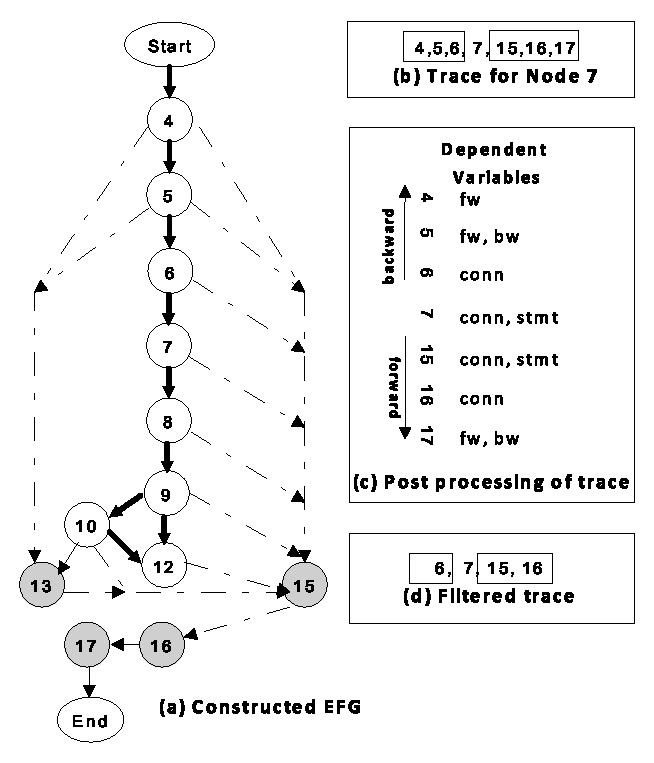
\includegraphics[scale=0.70,clip]{figs/forexamplesec1.eps}\vspace*{-2ex}
\caption{\label{fig:approchex} Illustrative examples of CAR-Miner approach.} \vspace*{-5ex}
\end{figure}

The frequent subsequence mining technique accepts a database of sequences such as $SDB_{1,2}$ and a minimum
support threshold \emph{min\_sup}, and returns subsequences that appear
at least \emph{min\_sup} times in the sequence database. 
Given a sequence \emph{s}, it is considered as frequent if
its support \emph{sup(s)} $\geq$ \emph{min\_sup}.
In our context, we are interested in frequent closed subsequences. A sequence \emph{s}
is a frequent closed sequence, if \emph{s} is frequent 
and no proper super sequence of \emph{s} is frequent. 
Figure~\ref{fig:condassorules}c shows an example 
closed frequent subsequence from the combined sequence database.
As sequence mining preserves temporal order among items, we
scan each closed frequent subsequence and transform the subsequence into an association rule
of the form ``\emph{X} $\Rightarrow$ \emph{Y}'' based on 
annotations (as shown in Figure~\ref{fig:condassorules}d).
We compute confidence values for each association rule  
using the formula as shown below:

\begin{CodeOut}
Confidence (\emph{X} $\Rightarrow$ \emph{Y}) = Support (\emph{X} \emph{Y}) / Support (\emph{X})
\end{CodeOut}

Although we explain our algorithm using two sequence databases $SDB_1$
and $SDB_2$, our algorithm can be applied to multiple sequence databases as well.
These multiple sequence databases can also be combined into 
a single sequence database using the similar mechanism illustrated in Figure~\ref{fig:condassorules}.

\vspace*{-2ex}
%--------------------------------------------------------------------------------------
\subsection*{Sequence Association Rules}
\vspace*{-2ex}
In our current approach, our target is to mine exception-handling rules in the form 
of association rules. Therefore, we collect two sequence databases for each function call $FC_a$:
a normal function-call-sequence (NFCS) database and an exception function-call-sequence (EFCS) database.
We apply our mining algorithm to generate sequence association rules 
of the form $FC_c^1$...$FC_c^n$ $\Rightarrow$ $FC_e^1$...$FC_e^m$, where
$FC_c^1$...$FC_c^n$ $\sqsubseteq$ $S_i$ $\in$ NFCS and $FC_e^1$...$FC_e^m$ $\sqsubseteq$
$S_j$ $\in$ EFCS.
Such an association rule describes that $FC_a$ should be followed by the 
function-call-sequence $FC_e^1$...$FC_e^m$ in exception paths, when preceded 
by the function-call-sequence $FC_c^1$...$FC_c^n$. 
As this association rule is specific to the function call
$FC_a$, we append $FC_a$ to the rule as
($FC_c^1$...$FC_c^n$) $\wedge$ $FC_a$ $\Rightarrow$ ($FC_e^1$...$FC_e^m$).
